\documentclass{standalone}
\usepackage{tikz}
\usepackage{amsmath}
\usetikzlibrary{matrix}
\begin{document}

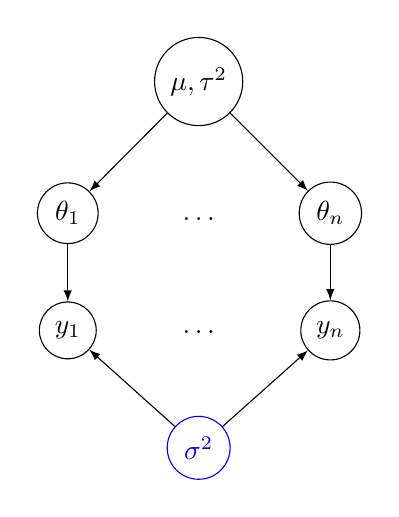
\begin{tikzpicture}[>=latex]
\matrix[matrix of math nodes, column sep=2em, row sep=2em,
        row 1 column 2/.style={nodes={circle, draw, minimum size=5mm}},
        every odd column/.style={nodes={circle, draw, minimum size=5mm}},
        row 4/.style={nodes={circle, draw, minimum size=5mm}}
       ] (mat)
{
    & \mu, \tau^2 & \\ 
    \theta_1 & \ldots & \theta_n \\
    y_1 & \ldots & y_n \\ 
    & |[blue]| \sigma^2 & \\
};

\foreach \column in {1, 3}
{
    \draw[->] (mat-1-2) -- (mat-2-\column);
    \draw[->] (mat-2-\column) -- (mat-3-\column);
    \draw[<-] (mat-3-\column) -- (mat-4-2);
}

\end{tikzpicture}
\end{document}
